Le circuit à implémenter pour connecter ce micro est donné à la Figure \ref{fig:circuit_H01}. Dans celui-ci, on retrouve la tension d'alimentation (\textsc{SUPPLY}) à 5V. Pour ce projet, nous utiliserons une alimentation réglable de laboratoire (si tu désires reproduire ce circuit chez toi, n'hésite pas à demander à un membre du staff quelle alimentation tu peux utiliser). Il te faudra également un micro et une résistance de 20k$\Omega$. 

\begin{figure}[!ht]
	\centering
	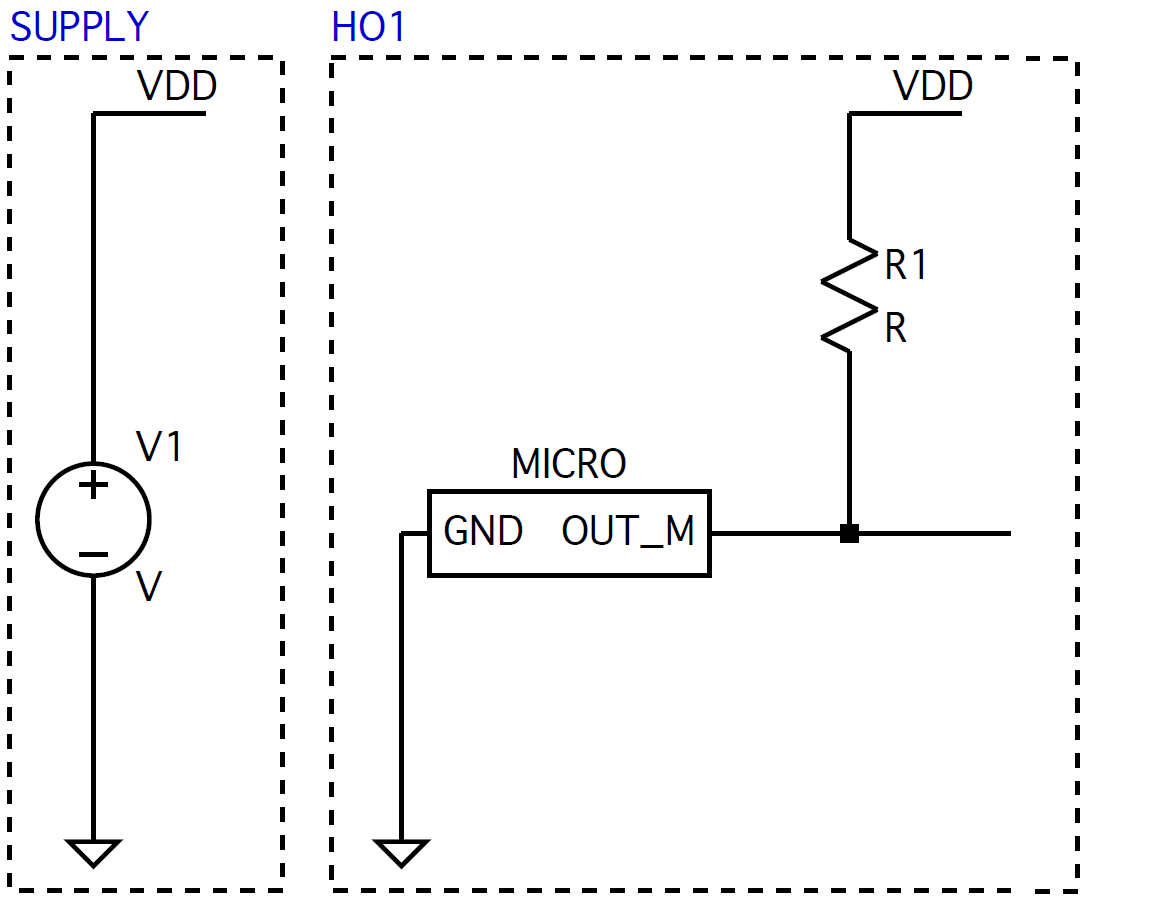
\includegraphics[width=.65\textwidth]{figures/circuit_1.png}
	\caption{Circuit HO1. $V1 = 5V$, $R1 = 20 k\Omega$}
	\label{fig:circuit_H01}
\end{figure}

Pour réaliser les connections, nous utiliserons une \textit{breadboard}. Ce sont des plaquettes qui permettent de facilement connecter et déconnecter des composants électroniques, bien pratiques pour effectuer des premiers tests. Pour l'utiliser, rien de plus simple: il suffit d'enfoncer les composants dans les trous de la plaquette en faisant en sorte de les placer correctement pour que les connections se fassent. Les trous de la plaquette sont connectés suivant le schéma de la Figure \ref{fig:breadboard}.

\begin{figure}[!ht]
	\centering
	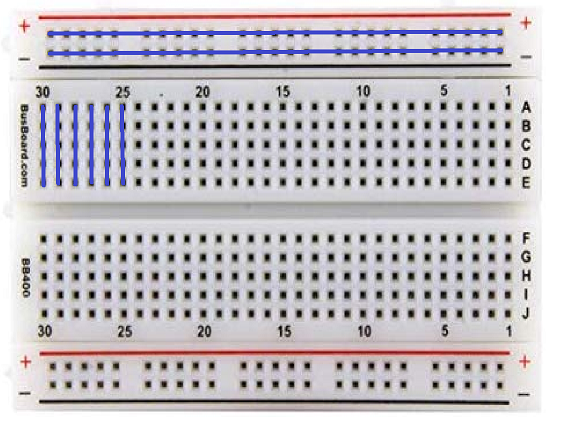
\includegraphics[width=.5\textwidth]{figures/breadboard.PNG}
	\caption{breadboard}
	\label{fig:breadboard}
\end{figure}
